\section{\index{arithmetic circuit}Arithmetic circuits}
\label{sec:circuits}

In this section we present the arithmetic circuit model and give some
classical results. Since we have in mind applications to the theory of
transposition, our presentation is slightly different from classical
presentations of the subject \cite{BuClSh, Vollmer}.

\begin{definition}[Arithmetic operator, arity]
  Let $R$ be a (non necessarily commutative) ring with unit. An
  arithmetic operator over $R$ is a function $f:R^i\ra R^o$ for some
  $i,o\in\N$.  Here $i$ is called the \emph{in-arity} of $f$ or simply
  \emph{arity}, $o$ is called the \emph{out-arity} of $f$.
\end{definition}

The exact meaning of the product $R^n$ varies depending on what is
meant by ``function'': a category must be specified in order for this
notions to be well defined. In this paper we will use two different
definitions:
\begin{itemize}
\item If we want ``function'' to mean any function in a set-theoretic
  sense, we work in the category $\mathsf{Set}$. Then $R^n$ is the
  product $\prod^nR$ of the category (the Cartesian product) and $R^0$
  is the terminal object of the category, i.e. any singleton. For
  convenience we note $\{\bom\}$ for $R^0$, with $\bom$ being its
  unique element.
\item In some cases it will be convenient to restrict ``function'' to
  mean ``morphism of left $R$-modules'', then we will work in the
  category $\RMod{R}$ of left $R$-modules with morphisms. Then $R^n$
  is the product $\prod^nR$ of the category and $R^0$ is the zero
  module.  We note $0$ for the zero module and $\bom$ for its unique
  element in order to avoid confusion with the $0$ of $R$ (and to
  stress the analogy with $\mathsf{Set}$). In what follows by
  ``module'' we will always mean ``left module''.
\end{itemize}

\begin{definition}[Arithmetic basis]
  Let $R$ be a ring.  An arithmetic $R$-basis is a (not necessarily
  finite) set of arithmetic operators over $R$.
\end{definition}

Two arithmetic bases will be important to us. The first one is the
\emph{standard basis}, noted $\Sbasis$. It is composed of the
following operators
\begin{equation}
  \label{eq:sbasis}
  \tag{$\Sbasis$}
  \begin{aligned}
    + : R\times R &\ra R    & * : R\times R &\ra R &  \hub : R &\ra R\times R\\
        a, b &\mapsto a+b   &     a, b &\mapsto ab &         a &\mapsto a,a\\ \\
    \eta_a : \{\bom\} &\ra R     &&& \omega : R &\ra \{\bom\} \\
          \bom &\mapsto a &&&          a &\mapsto \bom
  \end{aligned}
\end{equation}
Remark that $\eta_a$ defines a possibly infinite family of operators,
one for every $a\in R$.

The other one is the \emph{linear basis}, noted $\Tbasis$.  It
is composed of
\begin{equation*}
  \label{eq:tbasis}
  \tag{$\Tbasis$}
  \begin{aligned}
    + : R\times R &\ra R    &\quad
    \rmul{a} : R &\ra R      &\quad
    0 : 0 &\ra R  \\
    a, b &\mapsto a+b   &
    b &\mapsto ba &  
    \bom &\mapsto 0  \\
    \\
    \hub : R &\ra R\times R  &\quad
    &&
    \omega : R &\ra 0 \\
    a &\mapsto a,a    &
    &&
    a &\mapsto \bom
  \end{aligned}
\end{equation*}
The linear basis is reproduced in figure \ref{fig:nodes}.

Finally, the \emph{opposite linear basis}, noted $\Tbasis^\op$, is
obtained from $\Tbasis$ by substituting $\rmul{a}$ with
$\lmul{a}:b\mapsto ab$. Notice that this is just a shorthand notation
for the arithmetic $R^\op$-basis $\Tbasis$.

In terms of category theory, $\Sbasis$ only makes sense when working
with $\mathsf{Set}$, while $\Tbasis$ can be defined even when working
with $\RMod{R}$ (equivalently, $\Tbasis^\op$ can be defined when
working with $\ModR{R}$, the category of right $R$-modules).
\begin{figure}[!ht]
  \label{fig:nodes}
  \centering
  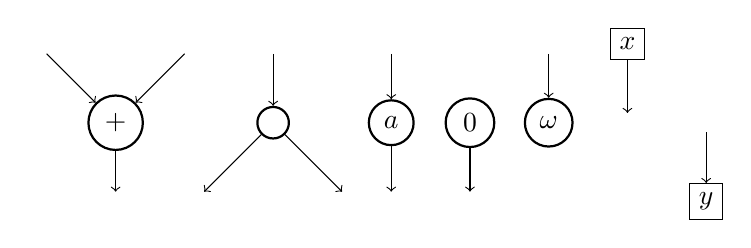
\begin{tikzpicture}
    \tikzstyle{node}=[circle,thick,draw=black,minimum size=4mm]
    \tikzstyle{arg}=[rectangle,thin,draw=black,minimum size=4mm]
    
    \begin{scope}
      \node(in1){};
      \node(nop)[right of=in1]{};
      \node(in2)[right of=nop]{};

      \node[node](plus)[below of=nop]{$+$};
      \node(out)[below of=plus]{};

      \path[->]
      (in1) edge (plus)
      (in2) edge (plus)
      (plus) edge (out);
    \end{scope}
    
    \begin{scope}[xshift=30mm]
      \node(in){};
      \node[node](hub)[below of=in]{$\hub$};
      \node(nop)[below of=hub]{};
      \node(out1)[left of=nop]{};
      \node(out2)[right of=nop]{};

      \path[->]
      (in) edge (hub)
      (hub) edge (out1)
      (hub) edge (out2);
    \end{scope}
    
    \begin{scope}[xshift=45mm]
      \node(in){};
      \node[node](times)[below of=in]{$\rmul{a}$};
      \node(out)[below of=times]{};

      \path[->]
      (in) edge (times)
      (times) edge (out);
    \end{scope}

    \begin{scope}[xshift=55mm]
      \node(nop){};
      \node[node][below of=nop](create){$0$};
      \node(out)[below of=create]{};
      \path[->] (create) edge (out);
    \end{scope}

    \begin{scope}[xshift=65mm]
      \node(in){};
      \node[node][below of=in](destroy){$\omega$};
      \node(nop)[below of=destroy]{};
      \path[->] (in) edge (destroy);
    \end{scope}

    \begin{scope}[xshift=75mm]
      \node[arg](in){$x$};
      \node[below of=in](out){};
      \path[->] (in) edge (out);
    \end{scope}

    \begin{scope}[xshift=85mm]
      \node(nop){};
      \node[below of=nop](in){};
      \node[arg](out)[below of=in]{$y$};
      \path[->] (in) edge (out);
    \end{scope}
  \end{tikzpicture}
  \caption{Nodes over the linear basis: round ones are evaluation
    nodes, square ones are input and output nodes.}
\end{figure}


Arithmetic circuits are directed acyclic multigraphs carrying
information from an arithmetic basis; the formal definition follows.

\begin{definition}[Arithmetic node]
  Let $R$ be a ring and $\mathcal{B}$ be an $R$-basis. A node over
  $(R,\mathcal{B})$ is a tuple $v=(I, O, f)$ such that
  \begin{itemize}
  \item $I$ and $O$ are finite ordered sets, 
  \item $f$ is either an element of $\mathcal{B}$ or the special value
    $\emptyset$.
  \item If $f=\emptyset$, one of the two following conditions must hold:
    \begin{itemize}
    \item $I$ is a singleton and $O$ is empty, in this case we say
      that $v$ is an \emph{input node};
    \item $I$ is empty and $O$ is a singleton, in this case we say
      that $v$ is an \emph{output node}.
    \end{itemize}
  \item If $f\ne\emptyset$, the cardinality of $I$ matches the
    in-arity of $f$ and the cardinality of $O$ matches the out-arity
    of $f$; in this case we say that $v$ is an \emph{evaluation node}.
  \end{itemize}
\end{definition}

We call \emph{input ports} the elements of $I$ and \emph{output ports}
the elements of $O$, we note respectively $\inp(v)$ and
$\outp(v)$. The cardinalities of $I$ and $O$ are called, respectively,
the \emph{in-degree} and \emph{out-degree} of $v$.  We call $f$ the
value of $v$ and note $\beta(v)$.

\begin{definition}[Arithmetic circuit]
  Let $R$ be a ring and $\mathcal{B}$ be an $R$-basis. An arithmetic
  circuit over $(R,\mathcal{B})$ is a tuple $C=(V,E)$ such that
  \begin{enumerate}
  \item $V$ is a finite ordered set of nodes over $(R,\mathcal{B})$,
  \item let $I=\biguplus_{v\in V}\inp(v)$ and $O=\biguplus_{v\in
      V}\outp(v)$, then $E$ is a bijection from $O$ to $I$.
  \end{enumerate}
\end{definition}

It is useful to see $E$ as a set of pairs $(o,i)$ with $i\in I$ and
$o\in O$. Then the elements of $E$ are called the \emph{edges} of the
circuit. The edges \emph{incident} to $v\in V$ are all the $(o,i)\in
E$ such that $i\in\inp(v)$; the edges \emph{stemming} from $v\in V$
are all the $(i,o)\in E$ such that $o\in\outp(v)$. An edge stemming
from $v$ and incident to $v'$ is said to \emph{connect} $v$ to $v'$.
We call \emph{inputs} and \emph{outputs} of a circuit, respectively,
the input and output nodes in $V$; we note $\inp(C)$ and $\outp(C)$.

By forgetting the ordering of $V$, a circuit induces a multiDAG with
labelled nodes, we call it the \emph{graph} of $C$. In what follows we
will often refer to graph-theoretic properties of the graph without
explicitly making the difference between a circuit and its graph.

Figure \ref{fig:circuit} shows an example of arithmetic circuit, the
analogy with multiDAGs is evident. We draw input and output nodes in
square boxes and evaluation nodes in round boxes. The orders on input
and output ports are implicitly represented by ordering edges
clockwise starting from 9 on the clock. The order on $V$ is actually
only important for input and output nodes: we implicitly represent
this information by arranging input and output nodes increasingly from
left to right, but we omit it for evaluation nodes. We will always use
these conventions when drawing circuits.

\begin{figure}[!ht] \centering
  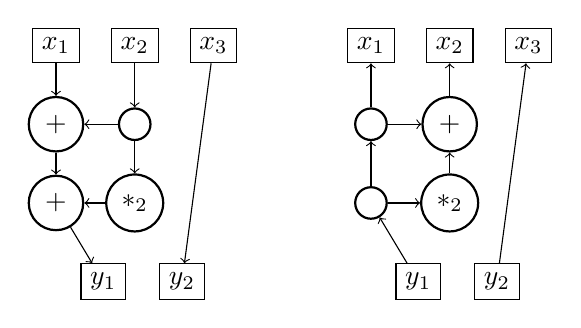
\begin{tikzpicture}
\tikzstyle{node}=[circle,thick,draw=black,minimum size=4mm]
\tikzstyle{arg}=[rectangle,thin,draw=black,minimum size=4mm]
    
    \begin{scope} \node[arg](in1){$x_1$}; \node[arg,right
of=in1](in2){$x_2$}; \node[arg,right of=in2](in3){$x_3$};
      
      \node[node,below of=in1](plus1){$+$}; \node[node,right
of=plus1](H){$\hub$};

      \node[node,below of=plus1](plus2){$+$}; \node[node,right
of=plus2](times){$*_2$};

      \node[arg,below of=plus2,xshift=6mm](out1){$y_1$};
\node[arg,right of=out1](out2){$y_2$};

      \path[->] (in1) edge (plus1) (in2) edge (H) (in3) edge (out2)
(H) edge (plus1) (H) edge (times) (plus1) edge (plus2) (times) edge
(plus2) (plus2) edge (out1);
    \end{scope}

    \begin{scope}[xshift=4cm]
      \node[arg](in1){$\dual{x_1}$};
      \node[arg,right of=in1](in2){$\dual{x_2}$};
      \node[arg,right of=in2](in3){$\dual{x_3}$};
      
      \node[node,below of=in1](plus1){$\hub$};
      \node[node,right of=plus1](H){$+$};

      \node[node,below of=plus1](plus2){$\hub$};
      \node[node,right of=plus2](times){$*_2$};

      \node[arg,below of=plus2,xshift=6mm](out1){$\dual{y_1}$};
      \node[arg,right of=out1](out2){$\dual{y_2}$};

      \path[<-]
      (in1) edge (plus1)
      (in2) edge (H)
      (in3) edge (out2)
      (H) edge (plus1)
      (H) edge (times) 
      (plus1) edge (plus2)
      (times) edge (plus2)
      (plus2) edge (out1);
    \end{scope}
  \end{tikzpicture}
  \caption{Two arithmetic circuits over $\Tbasis$. The linear map
    $y_1=x_1+3x_2, y_2=x_3$ is computed by the circuit on the left and
    its transpose is computed by the circuit on the right.}
  \label{fig:circuit}
\end{figure}

Circuits would be meaningless if they hadn't a semantic attached to
them. Intuitively the semantic corresponds to evaluation of the nodes
along the flow of the multiDAG.

\begin{definition}[Evaluation of an arithmetic circuit]
  \label{def:eval}
  Let $C$ be an arithmetic circuit with $i$ inputs and $o$ outputs,
  then its evaluation is a function $\eval_C:R^i\ra R^o$.

  In order to define it, we simultaneously define the evaluation
  $\eval_v$ of each $v\in V$ and the evaluation $\eval_e$ of each
  $e\in E$. We will note by $<_v$ the orders on the input and the
  output ports of $v$; we will also note by $<_V$ the order on $V$.
  \begin{itemize}
  \item Let $v\in V$ have out-degree $n$, let its evaluation be
    $\eval_v:R^i\ra R^n$ and let $\pi_1,\ldots,\pi_n$ be the canonical
    projections from $R^n$ to $R$. Let $o_1<_v\cdots<_vo_n$ be the
    output ports of $v$ and let $e_j=\bigl(o_j,E(o_j)\bigr)$ be the
    corresponding edges stemming from $v$, then $\eval_{e_j} =
    \pi_j\circ\eval_v$ for any $j$.
  \item Let $x_1<_V\cdots<_Vx_n$ be the input nodes and let
    $\pi_1,\ldots,\pi_i$ be the canonical projections from $R^i$ to
    $R$, then $\eval_{x_j}=\pi_j$ for any $j$.
  \item For every evaluation node $v$ with in-degree $m$, let
    $i_1<_v\cdots<_vi_m$ be the input ports of $v$ and let
    $e_j=\bigl(E^{-1}(i_j),i_j\bigr)$ be the corresponding edges
    incident to $v$, then
    \begin{equation}
      \label{eq:eval_v}
      \eval_v = \beta(v) \circ (\eval_{e_1} \times \cdots \times \eval_{e_m})
      \text{.}
    \end{equation}
  \item For every output node $y$, let $e\in E$ be the only edge
    incident to $y$, then $\eval_y=\eval_e$.
  \end{itemize}

  We can finally define $\eval_C:R^i\ra R^o$. Let $y_1<_V\cdots<_Vy_o$
  be the output nodes, then
  \begin{equation}
    \label{eq:eval}
    \eval_C = \eval_{y_1} \times \cdots \times \eval_{y_o}
    \text{.}
  \end{equation}
  We also say that $C$ \emph{computes} $\eval_C$.
\end{definition}

Observe that the products of functions in equation \eqref{eq:eval_v}
and \eqref{eq:eval} are formally defined via the universal property of
the product: for any collection of functions $f_j:X\ra R$, the product
$f=\prod_jf_j$ is the unique function $f:X\ra \prod_jR$ such that
$f_j=\pi_j\circ f$ for any $j$. This allows us to easily show the
following property.

\begin{proposition}
  The evaluation of an arithmetic circuit is an arrow (a function) in
  the category of interest. In particular, the evaluation of a circuit
  over $(R,\Tbasis)$ is a morphism of $R$-modules.
\end{proposition}

The converse is not necessarily true : not any arrow of the category
can be computed by a circuit. However for the basis $\Tbasis$ it is
possible to give a partial converse.

\begin{proposition}
  Any morphism of free finite-dimensional $R$-modules can be computed
  by an arithmetic circuit over $(R,\Tbasis)$.
\end{proposition}
\begin{proof}
  Take the matrix associated to such morphism and create a circuit
  that performs the matrix-vector product.
\end{proof}

Circuits can be composed in a natural way by connecting their inputs
and outputs.

\begin{definition}[Composition of circuits]
  Let $C=(V,E)$ and $C'=(V',E')$ be two circuits over
  $(R,\mathcal{B})$ and let $\mathcal{R}:\outp(C)\ra\inp(C')$ be an injective
  partial function. The composition of $C$ and $C'$ through
  $\mathcal{R}$, noted $C'\overset{\mathcal{R}}{\circ}C$, is the
  circuit $(V'', E'')$ such that
  \begin{itemize}
  \item $V'' = \bigr(V - \mathcal{R}^{-1}(\inp(C'))\bigr) \uplus
    \bigl(V' - \mathcal{R}(\outp(C))\bigr)$ with the orders inherited
    from $V$ and $V'$ and the supplementary condition that $v<v'$
    whenever $v\in V$ and $v'\in V'$.
  \item $E''(o) = \begin{cases}
      E'(o') & \text{if $E(o)\in\inp(v')$ and $\mathcal{R}(v') = v''$ and $\outp(v'')=\{o'\}$,}\\
      (E\uplus E')(o) & \text{otherwise.}
    \end{cases}$
  \end{itemize}

  When the function $\mathcal{R}$ is total, bijective and monotone
  (w.r.t. the orders on $V$ and $V'$), we say the the composition is
  \emph{natural} and simply note $C'\circ C$.
\end{definition}


\begin{figure}[!ht] \centering
  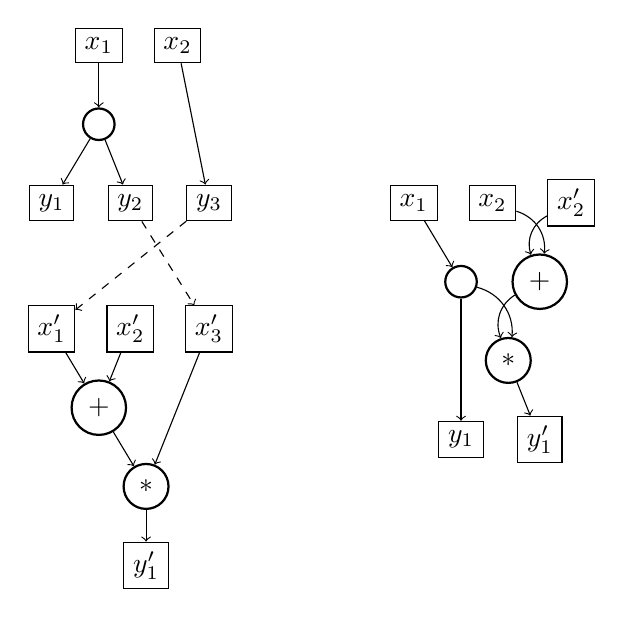
\begin{tikzpicture}
    \tikzstyle{node}=[circle,thick,draw=black,minimum size=4mm]
    \tikzstyle{arg}=[rectangle,thin,draw=black,minimum size=4mm]
    
    \begin{scope}
      \node[arg](in1){$x_1$};
      \node[arg,right of=in1](in2){$x_2$};
      
      \node[node,below of=in1](H){$\hub$};

      \node[arg,below of=H, xshift=-6mm](out1){$y_1$};
      \node[arg,right of=out1](out2){$y_2$};
      \node[arg,right of=out2](out3){$y_3$};

      \path[->]
      (in1) edge (H)
      (in2) edge (out3)
      (H) edge (out1)
      (H) edge (out2);

      \node[arg,below of=out1,yshift=-6mm](in3){$x'_1$};
      \node[arg,right of=in3](in4){$x'_2$};
      \node[arg,right of=in4](in5){$x'_3$};

      \node[node,below of=in3,xshift=6mm](plus1){$+$};
      
      \node[node,below of=plus1,xshift=6mm](plus2){$*$};

      \node[arg,below of=plus2](out4){$y'_1$};

      \path[->]
      (in3) edge (plus1)
      (in4) edge (plus1)
      (plus1) edge (plus2)
      (in5) edge (plus2)
      (plus2) edge (out4);

      \path[->,dashed]
      (out2) edge (in5)
      (out3) edge (in3);
    \end{scope}

    \begin{scope}[xshift=3cm,yshift=-3cm]
      \Large
      \node(=>){$\Ra$};
    \end{scope}

    \begin{scope}[xshift=4cm,yshift=-2cm]
      \node[arg](in1){$x_1$};
      \node[arg,right of=in1](in2){$x_2$};
      \node[arg,right of=in2](in4){$x'_2$};
      
      \node[node,below of=in1,xshift=6mm](H){$\hub$};

      \node[node,below of=in2,xshift=6mm](plus1){$+$};
      
      \node[node,below of=plus1, xshift=-4mm](plus2){$*$};

      \node[arg,below of=plus2,xshift=4mm](out4){$y'_1$};
      \node[arg,left of=out4](out1){$y_1$};

      \path[->]
      (in1) edge (H)
      (in2) edge[bend left=40] (plus1)
      (H) edge[bend left=40] (plus2)
      (H) edge (out1);

      \path[->]
      (in4) edge[bend right=40] (plus1)
      (plus1) edge[bend right=40] (plus2)
      (plus2) edge (out4);
    \end{scope}
  \end{tikzpicture}
  \caption{Composition of circuits through $\mathcal{R} = \{y_2\mapsto
    x'_3, y_3\mapsto x'_1\}$.}
  \label{fig:composition}
\end{figure}
An example of composition is given in figure \ref{fig:composition}.
It is evident that the concept of natural composition coincides with
composition of functions, the proof of the following proposition is
trivial.

\begin{proposition}
  Let $C$ and $C'$ be circuits over $(R,\mathcal{B})$ and let $C$
  have as many outputs as $C'$ has inputs, then
  \[\eval_{C'\circ C} = \eval_{C'}\circ\eval_{C} \text{.}\]
\end{proposition}

Another evidence that we state without proof is the fact that any
circuit over $(R,\mathcal{B})$ can be obtained by composition of small
elementary circuits.

\begin{proposition}
  We call \emph{elementary} a circuit that has one unique evaluation
  node. Any circuit can be obtained by composition of elementary
  circuits.
\end{proposition}

We finally define a way of substituting nodes, first syntactically,
then semantically.

\begin{definition}[Syntactic substitution]
  Let $C=(V,E)$ be a circuit over $(R,\mathcal{B})$ and let
  $C'=(V',E')$ be a circuit over $(R,\mathcal{B}')$. Let $C'$ have $i$
  inputs and $o$ outputs and let $v\in V$ have in-degree $i$ and
  out-degree $o$. 

  Let $\mathcal{I}$ and $\mathcal{O}$ be monotone bijections
  respectively from $\inp(v)$ to $\inp(C')$ and from $\outp(C')$ to
  $\outp(v)$. We note by $C[C'/v]$ the circuit $(V'',E'')$ over
  $(R,\mathcal{B}\cup\mathcal{B}')$ defined as follows:
  \begin{itemize}
  \item $V'' = V\uplus (V' - \inp(C') - \outp(C'))$,
  \item $E''(o) = \begin{cases}
      E'(o') & \text{if $E(o)\in\inp(v)$ and $\mathcal{I}(E(o))=v'$ and $\outp(v')=\{o'\}$,}\\
      E(o') & \text{if $E'(o)\in\outp(C')$ and $\mathcal{O}(E'(o))=o'$,}\\
      (E\uplus E')(o) & \text{otherwise.}
    \end{cases}$
  \end{itemize}
\end{definition}

\begin{definition}[Semantic substitution]
  Let $C$ be a circuit over $(R,\mathcal{B}\cup\{f\})$ and let $F$ be
  a circuit over $(R,\mathcal{B})$ such that $\eval_F=f$.

  We note by $C[F/f]$ the circuit over $(R,\mathcal{B})$ where any
  node $v$ of $C$ such that $\beta(v)=f$ has been syntactically
  substituted by $F$.

  It is obvious that
  \[\eval_{C[F/f]} = \eval_C \text{.}\]
\end{definition}

As a shorthand notation, we will draw octogones to signify that a node
has been syntactically substituted by a circuit, without giving the
actual shape of the substituting circuit. Figure
\ref{fig:substitution} shows an example.

\begin{figure}[!ht]
  \label{fig:substitution}
  \centering
  \begin{tikzpicture}
    \tikzstyle{node}=[circle,thick,draw=black,minimum size=4mm]
    \tikzstyle{arg}=[rectangle,thin,draw=black,minimum size=4mm]
    \tikzstyle{subst}=[regular polygon,regular polygon sides=8,thick,draw=black,minimum size=4mm]
    
    \begin{scope}
      \node[arg](in1){$x_1$};
      \node[arg,right of=in1](in2){$x_2$};
      
      \node[node](H)[below of=in2]{$\hub$};
      \node[subst](F)[left of=H]{$F$};

      \node[arg,below of=F,xshift=-6mm](out1){$y_1$};
      \node[arg,right of=out1](out2){$y_2$};
      \node[arg,right of=out2](out3){$y_3$};

      \path[->]
      (in1) edge (F)
      (in2) edge (H)
      (H) edge[bend left=10] (F)
      (H) edge[bend right=10] (F)
      (F) edge (out1)
      (F) edge (out2)
      (F) edge (out3);
    \end{scope}

  \end{tikzpicture}
  \caption{Arithmetic circuit where a node has been syntactically
    substituted by a circuit $F$ with $3$ inputs and $3$ outputs.}
\end{figure}

This shows that circuits are a good formalism to describe
functions. However, they carry more information than simply their
evaluation; the next step is to classify them in a
complexity-theoretic way.

\begin{definition}[Size, depth]
  \label{def:size}
  Let $C$ be a circuit over $(R,\mathcal{B})$. The size of $C$, noted
  $\size(C)$ is the number of evaluation nodes in $V$; the depth of
  $C$, noted $\depth(C)$ is the length of the longest directed path
  --in a graph-theoretic sense-- in $(V,E)$.

  Sometimes it is useful to only count certain nodes. Let
  $X\subset\mathcal{B}$, the $X$-weighted size of $C$, noted
  $\size_X(C)$ is the number of nodes $v\in V$ such that $\beta(v)\in
  X$.
\end{definition}


\subsection{Coevaluation}
When dealing with a construction in category theory, it is natural to
simultaneously study its dual, that is the construction obtained by
\emph{reversing all the arrows}. If in definition \ref{def:eval} we
substitute the product $\prod^nR$ by its dual $\coprod^nR$, called
\emph{coproduct}, we obtain a new way of evaluating an arithmetic
circuit that we will call \emph{coevaluation}. We study here the
properties of coevaluation, its interest will be clear in the next
sections.

In this context, we will make an abuse by using the same notation
$R^n$ we used for the product to signify the coproduct $\coprod^nR$ in
the category. Whether $R^n$ is product or coproduct will always be
clear from the context.

\begin{definition}[Arithmetic co-operator, cobasis]
  Let $R$ be a ring. An arithmetic co-operator over $R$ is a function
  $f:R^i\ra R^o$ for some $i,o\in\N$; here $R^n$ is coproduct.

  An arithmetic $R$-cobasis is a set of arithmetic co-operators over
  $R$.
\end{definition}

In particular when the category is $\mathsf{Set}$ the coproduct is the
disjoint union of sets, thus the bases $\Sbasis$ and $\Tbasis$ make no
sense in this context.

The definitions of node and circuit naturally extend to cobases, but
we need to define a new evaluation for arithmetic circuits defined
over them.

\begin{definition}[coevaluation of an arithmetic circuit]
  \label{def:coeval}
  Let $C$ be an arithmetic circuit with $i$ inputs and $o$ outputs
  over a cobasis $\mathcal{B}$. Its coevaluation is a function
  $\lave_C:R^i\ra R^o$.

  We use the same notation as in definition \ref{def:eval}. As we did
  there, we simultaneously define $\lave_v$ for each $v\in V$ and
  $\lave_e$ for each $e\in E$.
  \begin{itemize}
  \item Let $v\in V$ have in-degree $m$, let its coevaluation be
    $\lave_v:R^m\ra R^o$ and let $\iota_1,\ldots,\iota_n$ be the
    canonical injections from $R$ to $R^m$. Let $i_1<_v\cdots<_vi_m$
    be the input ports of $v$ and let
    $e_j=\bigl(i_j,E^{-1}(i_j)\bigr)$ be the corresponding edges
    incident to $v$, then $\lave_{e_j} = \lave_v\circ\iota_j$ for any
    $j$.
  \item Let $y_1<_V\cdots<_Vy_n$ be the output nodes and let
    $\iota_1,\ldots,\iota_o$ be the canonical injections from $R$ to
    $R^o$, then $\lave_{y_j}=\iota_j$ for any $j$.
  \item For every evaluation node $v$ with out-degree $n$, let
    $o_1<_v\cdots<_vo_n$ be the output ports of $v$ and let
    $e_j=\bigl(E(o_j),o_j\bigr)$ be the corresponding edges
    stemming from $v$, then
    \begin{equation}
      \label{eq:lave_v}
      \lave_v = (\lave_{e_1} \oplus \cdots \oplus \lave_{e_n}) \circ \beta(v) 
      \text{.}
    \end{equation}
  \item For every input node $x$, let $e\in E$ be the only edge
    stemming from $x$, then $\lave_x=\lave_e$.
  \end{itemize}

  We can finally define $\lave_C:R^i\ra R^o$. Let $x_1<_V\cdots<_Vx_i$
  be the input nodes, then
  \begin{equation}
    \label{eq:lave}
    \lave_C = \lave_{x_1} \oplus \cdots \oplus \lave_{x_i}
    \text{.}
  \end{equation}
\end{definition}

As before, the sums of equations \eqref{eq:lave_v} and \eqref{eq:lave}
are formally defined via the universal property of the coproduct.

The coevaluation in general does not attach the same semantics to a
circuit as the evaluation. For example in the case of $\mathsf{Set}$
the coevaluation is a function from the disjoint union of $i$ copies
of $R$ to the disjoint union of $o$ copies of $R$. We can regard
circuits over cobases in $\mathsf{Set}$ as objects that are fed one
single element of $R$ on one out of their $n$ inputs and then take
decisions depending on which input was fed. An example is given in
figure \ref{fig:coffee}.

\begin{figure}[!ht]
  \centering
  
  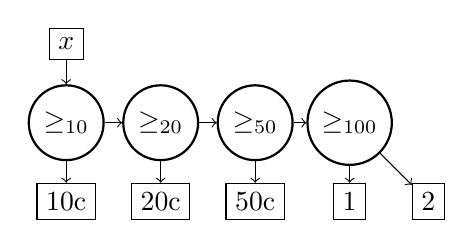
\begin{tikzpicture}
    \tikzstyle{node}=[circle,thick,draw=black,minimum size=4mm]
    \tikzstyle{arg}=[rectangle,thin,draw=black,minimum size=4mm]

    \begin{scope}
      \node[arg](in){$x$};

      \node[node,below of=in](s10){$\ge_{10}$};

      \node[node,right of=s10,xshift=2mm](s20){$\ge_{20}$};
      \node[arg,below of=s10](o10){$10$c};

      \node[node,right of=s20,xshift=2mm](s50){$\ge_{50}$};
      \node[arg,below of=s20](o20){$20$c};

      \node[node,right of=s50,xshift=2mm](s1){$\ge_{100}$};
      \node[arg,below of=s50](o50){$50$c};

      \node[arg,below of=s1](o1){$1$\euro};
      \node[arg,right of=o1](o2){$2$\euro};

      \path[->]
      (in) edge (s10)
      (s10) edge (o10)
      (s10) edge (s20)
      (s20) edge (o20)
      (s20) edge (s50)
      (s50) edge (o50)
      (s50) edge (s1)
      (s1) edge (o1)
      (s1) edge (o2);
    \end{scope}
  \end{tikzpicture}  
  
  \caption{The coffee machine circuit. On input $r\in R$, the operator
    $\ge_x:R\ra R\uplus R$ gives $r$ on its first output if $r\ge x$, on its
    second output otherwise. The circuit is an euro coin separator.}
  \label{fig:coffee}
\end{figure}

In some cases, howevever, evaluation and coevaluation coincide. The
following lemma shows one important case when this happens.

\begin{lemma}
  \label{th:coeval}
  Let $C$ be a circuit over $(R,\Tbasis)$. In the category $\RMod{R}$
  $\eval_C\simeq\lave_C$.
\end{lemma}
\begin{proof}
  For finite dimensional modules, the product and the direct sum are
  the same object. More formally, when working in $\RMod{R}$ there is
  a natural isomorphism $\prod^n R\simeq\coprod^n R$ for any $n$ (this
  is true for any additive category, see \cite[VIII.2]{McLane}). Thus
  $\Tbasis$ is both a basis and a cobasis, up to isomorphism, and both
  evaluation and coevaluation of circuits over it are meaningful.

  The rest of the proof is just induction on the size of the
  circuit. First, it is obvious that for elementary circuits with an
  unique evaluation node $v$ we have $\eval_C \simeq \beta(v) \simeq
  \lave_C$. Then it suffices to show that the property is maintained
  upon composition of circuits.
\end{proof}

The equivalence of evaluations and coevalutions suggests that there is
some unexploited symmetry in circuits over $\Tbasis$. The next
section explores it.


\subsection{The transposition theorem}
\label{sec:tellegen}

Since we are in a non-commutative setting, we have to precisely define
what we mean by ``transposition''. We start by recalling some well
known facts.


The transposition theorem says that from a circuit that computes the
matrix-vector product $x\mapsto \trans{x}M$ for a fixed matrix $M$, one can
deduce another circuit that computes $y\mapsto My$. We now
give such construction.

\begin{definition}[Dual circuit]
  \label{def:dual}
  Let $C=(V,E)$ be a circuit over $(R,\Tbasis)$, the dual circuit of
  $C$, noted $\dual{C}$, is the arithmetic circuit $\dual{C} = (V',
  E)$ over $(R^{\op},\Tbasis)$ where for any node $v=(I,O,f)$ in $V$
  there is a node $\dual{v}=(O,I,f')$ in $V'$ where
  \begin{equation}
    \label{eq:dual-circuit}
    f' = \begin{cases}
      \rmul{a} & \text{if $f = \rmul{a^\op}$}\\
      + & \text{if $f = \hub$}\\
      \hub & \text{if $f = +$}\\
      \omega & \text{if $f = 0$}\\
      0 & \text{if $f = \omega$}
    \end{cases}
  \end{equation}
  The ordering of $V'$ is the same as the one of $V$.
\end{definition}

In particular, this makes $(V',E)$ the reverse graph of $(V,E)$ in a
graph-theoretic sense. Figure \ref{fig:circuit} shows two circuits
that are each other's dual.

\begin{theorem}[Transposition theorem, Fiduccia '72]
  \label{th:tellegen}
  Let $C$ be a circuit over $(R,\Tbasis)$ that computes a module
  homomorphism $f$, then $\dual{C}$ computes the dual homomorphism
  $\dual{f}$.
\end{theorem}
\begin{proof}
  We apply the functor $\dual{()}$ to the construction of $\eval_C$ as
  defined in \ref{def:eval}. It is routine to verify that
  \begin{itemize}
  \item canonical projections in $\RMod{R}$ are taken to canonical
    injections in $\RMod{R^\op}$;
  \item products are taken to coproducts, in particular
    $\dual{\left(\prod^n R\right)} \simeq \coprod^nR^\op$ and the isomorphism is canonical;
  \item any morphism $t\in\Tbasis$ is taken it to its dual $\dual{t}$
    in $\Tbasis^\op$, the same correspondences as in equation
    \eqref{eq:dual-circuit} hold.
  \end{itemize}
  Furthermore, since $\dual{()}$ is contravariant, all the arrows are
  reversed. By comparing this with definitions \ref{def:coeval} and
  \ref{def:dual}, we clearly see that up to a natural isomorphism
  $\dual{\eval_C}\simeq\lave_{\dual{C}}$.

  The claim follows from lemma \ref{th:coeval}.
\end{proof}

\begin{corollary}
  A linear function $f:R^n\ra R^m$ and its dual can be computed by
  arithmetic circuits of same sizes and depths. In particular if $C$
  computes $f$ and $\dual{C}$ computes $\dual{f}$,
  \begin{gather*}
    \size_{\{+\}}(C) = \size_{\{\hub\}}(\dual{C}), \qquad  
    \size_{\{\hub\}}(C) = \size_{\{+\}}(\dual{C}), \\
    \size_{\{\rmul{a}\}}(C) = \size_{\{\rmul{a}\}}(\dual{C})\quad\text{for any $a\in R$},\\
    \size_{\{0\}}(C) = \size_{\{\omega\}}(\dual{C}), \qquad 
    \size_{\{\omega\}}(C) = \size_{\{0\}}(\dual{C}).
  \end{gather*}
\end{corollary}

In the commutative world, if $M$ is the matrix associated to the
homomorphism $f$, $\trans{M}$ is the matrix associated to $\dual{f}$
(up to isomorphism), but when $R$ is not commutative
$\trans{(AB)}\ne\trans{B}\trans{A}$ and this correspondence fails. We
can nevertheless define another transformation on circuits that acts
in a way similar to transposition in some special cases.

\begin{definition}[Opposite circuit]
  Let $C=(V,E)$ be a circuit over $(R,\Tbasis)$, the \emph{opposite
    circuit} of $C$, noted $C^\op$, is the arithmetic circuit over
  $(R^{\op},\Tbasis)$ where any $\beta(v)=\rmul{a}$ has been changed to $\rmul{a^\op}$.
\end{definition}

Now the opposite of a circuit certainly computes some $R^\op$-module
homomorphism, but there is no unique relationship between $\eval_C$
and $\eval_{C^\op}$ due to the lack of commutativity. A special case
of interest is stated in the next corollary.

\begin{definition}[Bilinear chain]
  Let $R$ be non-commutative and let $S\subset R$ be a subring of its
  center. A circuit $C$ over $(R,\Tbasis)$ such that no directed path
  in $C$ contains two nodes $v\ne v'$ with $\beta(v)=\rmul{a}$ and
  $\beta(v')=\rmul{a'}$ where $a,a'\not\in S$ is called an
  $S$-\emph{bilinear chain}.
\end{definition}

\begin{corollary}
  Let $C$ be a bilinear chain and let $\eval_C(x)=\trans{x}M$ for some
  matrix $M$, then $\eval_{C^\op}(x)=\trans{M}x$.
\end{corollary}
\begin{proof}
  Let $x_1,\ldots,x_n$ be the inputs of $C$ and $y_1,\ldots,y_m$ its
  outputs and let $M$ be the $n\times m$ matrix associated to
  $\eval_C$. Each path connecting $x_i$ to $y_j$ contributes linearly
  to the entry $(M)_{i,j}$; more precisely, let $p$ be a path from
  $x_i$ to $y_j$ and let $\rmul{a_1},\ldots,\rmul{a_h}$ be the
  multiplication nodes appearing (in that order) on it, we associate
  to $p$ the element $C_p=a_1\cdots a_h\in R$, then
  \begin{equation}
    (M)_{i,j}=\sum_{p\in\mathcal{P}(x_i,x_j)}C_p
  \end{equation}
  where $p$ ranges over the paths from $x_i$ to $x_j$. Obviously, to
  any path in $C$ corresponds an unique path in $C^\op$, by nothing
  them with the same letter $p$ we have
  \begin{equation}
    C_p^\op=a_1^\op\cdots a_n^\op=(a_n\cdots a_1)^\op=(C_p)^\op
    \text{ ,}
  \end{equation}
  where the last equality comes from the fact that all the $a_i$
  except at most one are in the center of $R$. We conclude that if
  $M'$ is the matrix associated to $C^\op$ then
  \begin{equation}
    (M')_{i,j}=\sum_{p\in\mathcal{P}(x_i,x_j)}C_p^\op=(M)_{i,j}^\op
    \text{ ;}
  \end{equation}
  and thus $\trans{x}M'=\trans{\left(\trans{M}x\right)}$.
\end{proof}



\subsection{Uniformity}
\label{sec:uniformity}

A circuit is limited to compute one specific function with inputs and
outputs of fixed size (in term of elements of $R$). However complexity
theory is interested in algorithms that compute on inputs of variable
size. This will lead us to study families of circuits.

\begin{definition}[Circuit family]
  Let $R$ be a ring, $\mathcal{B}$ a basis over $R$ and $\pspace$ a
  set. A \emph{circuit family} over $(R,\mathcal{B},\pspace)$ is a
  family of circuits over $(R,\mathcal{B})$ indexed by $\pspace$.
  $\pspace$ is called the \emph{parameter space} of the family.
\end{definition}

Algebraic complexity textbooks usually take $\pspace=\N$ and force
$C_n$ to have $n$ inputs. Our construction is more general and its
interest will be clear in the next sections.

\begin{definition}[Size and depth functions]
  Let $\mathcal{C} = (C_j)_{j\in\pspace}$ be a circuit family, we
  define the size and depth function as
  \begin{align*}
    \size^{\mathcal{C}}:\pspace&\ra\N  & \depth^{\mathcal{C}}:\pspace&\ra\N\\
                   j&\mapsto\size(C_j) &    j&\mapsto\depth(C_j)
  \end{align*}
  respectively.

  As in definition \ref{def:size}, for $X\subset\mathcal{B}$ we also
  define
  \begin{align*}
    \size^{\mathcal{C}}_X:\pspace&\ra\N\\
                     j&\mapsto\size_X(C_j)
                     \text{ .}
  \end{align*}
\end{definition}

Circuit families are interesting in theory and theorem
\ref{th:tellegen} easily generalizes to them. However this model of
computation is strictly more powerful than the BSS one (see \cite[Obs.
2.3]{Vollmer}). It is sometimes desirable to restrict oneself to a
more constrained model.

\begin{definition}[Uniform circuit family]
  Let $\mathcal{C} = (C_j)_{j\in\pspace}$ be a circuit family. Fix a
  binary representation of arithmetic circuits over $(R,\mathcal{B})$
  and a binary representation of $\pspace$.

  $\mathcal{C}$ is said to be uniform if there is a multi-band Turing
  machine $\mathcal{M}$ that on input $x$ writes the binary
  representation of $C_x$ on its output tape if $x$ is the binary
  representation of an element of $\pspace$, or an error token otherwise.

  The complexity of $\mathcal{M}$ is called the \emph{uniform
    complexity} of $\mathcal{C}$.
\end{definition}

We are mainly interested in uniform circuit families since they are
equivalent to computable functions, theorem \ref{th:tellegen} easily
generalizes to them. We won't study uniform circuit families more in
depth. Instead, we directly work on computer programs that implicitly
represent circuit families, and automatically deduce the transposed
family without actually using the circuit model. More details on
uniform circuit families can be found in \cite{Vollmer}.



% Local Variables:
% mode:flyspell
% ispell-local-dictionary:"american"
% mode:TeX-PDF
% mode:reftex
% TeX-master: "../these"
% End:
%
